% Options for packages loaded elsewhere
\PassOptionsToPackage{unicode}{hyperref}
\PassOptionsToPackage{hyphens}{url}
\PassOptionsToPackage{dvipsnames,svgnames,x11names}{xcolor}
%
\documentclass[
  letterpaper,
]{krantz}

\usepackage{amsmath,amssymb}
\usepackage{iftex}
\ifPDFTeX
  \usepackage[T1]{fontenc}
  \usepackage[utf8]{inputenc}
  \usepackage{textcomp} % provide euro and other symbols
\else % if luatex or xetex
  \usepackage{unicode-math}
  \defaultfontfeatures{Scale=MatchLowercase}
  \defaultfontfeatures[\rmfamily]{Ligatures=TeX,Scale=1}
\fi
\usepackage{lmodern}
\ifPDFTeX\else  
    % xetex/luatex font selection
\fi
% Use upquote if available, for straight quotes in verbatim environments
\IfFileExists{upquote.sty}{\usepackage{upquote}}{}
\IfFileExists{microtype.sty}{% use microtype if available
  \usepackage[]{microtype}
  \UseMicrotypeSet[protrusion]{basicmath} % disable protrusion for tt fonts
}{}
\makeatletter
\@ifundefined{KOMAClassName}{% if non-KOMA class
  \IfFileExists{parskip.sty}{%
    \usepackage{parskip}
  }{% else
    \setlength{\parindent}{0pt}
    \setlength{\parskip}{6pt plus 2pt minus 1pt}}
}{% if KOMA class
  \KOMAoptions{parskip=half}}
\makeatother
\usepackage{xcolor}
\setlength{\emergencystretch}{3em} % prevent overfull lines
\setcounter{secnumdepth}{5}
% Make \paragraph and \subparagraph free-standing
\ifx\paragraph\undefined\else
  \let\oldparagraph\paragraph
  \renewcommand{\paragraph}[1]{\oldparagraph{#1}\mbox{}}
\fi
\ifx\subparagraph\undefined\else
  \let\oldsubparagraph\subparagraph
  \renewcommand{\subparagraph}[1]{\oldsubparagraph{#1}\mbox{}}
\fi

\usepackage{color}
\usepackage{fancyvrb}
\newcommand{\VerbBar}{|}
\newcommand{\VERB}{\Verb[commandchars=\\\{\}]}
\DefineVerbatimEnvironment{Highlighting}{Verbatim}{commandchars=\\\{\}}
% Add ',fontsize=\small' for more characters per line
\usepackage{framed}
\definecolor{shadecolor}{RGB}{241,243,245}
\newenvironment{Shaded}{\begin{snugshade}}{\end{snugshade}}
\newcommand{\AlertTok}[1]{\textcolor[rgb]{0.68,0.00,0.00}{#1}}
\newcommand{\AnnotationTok}[1]{\textcolor[rgb]{0.37,0.37,0.37}{#1}}
\newcommand{\AttributeTok}[1]{\textcolor[rgb]{0.40,0.45,0.13}{#1}}
\newcommand{\BaseNTok}[1]{\textcolor[rgb]{0.68,0.00,0.00}{#1}}
\newcommand{\BuiltInTok}[1]{\textcolor[rgb]{0.00,0.23,0.31}{#1}}
\newcommand{\CharTok}[1]{\textcolor[rgb]{0.13,0.47,0.30}{#1}}
\newcommand{\CommentTok}[1]{\textcolor[rgb]{0.37,0.37,0.37}{#1}}
\newcommand{\CommentVarTok}[1]{\textcolor[rgb]{0.37,0.37,0.37}{\textit{#1}}}
\newcommand{\ConstantTok}[1]{\textcolor[rgb]{0.56,0.35,0.01}{#1}}
\newcommand{\ControlFlowTok}[1]{\textcolor[rgb]{0.00,0.23,0.31}{#1}}
\newcommand{\DataTypeTok}[1]{\textcolor[rgb]{0.68,0.00,0.00}{#1}}
\newcommand{\DecValTok}[1]{\textcolor[rgb]{0.68,0.00,0.00}{#1}}
\newcommand{\DocumentationTok}[1]{\textcolor[rgb]{0.37,0.37,0.37}{\textit{#1}}}
\newcommand{\ErrorTok}[1]{\textcolor[rgb]{0.68,0.00,0.00}{#1}}
\newcommand{\ExtensionTok}[1]{\textcolor[rgb]{0.00,0.23,0.31}{#1}}
\newcommand{\FloatTok}[1]{\textcolor[rgb]{0.68,0.00,0.00}{#1}}
\newcommand{\FunctionTok}[1]{\textcolor[rgb]{0.28,0.35,0.67}{#1}}
\newcommand{\ImportTok}[1]{\textcolor[rgb]{0.00,0.46,0.62}{#1}}
\newcommand{\InformationTok}[1]{\textcolor[rgb]{0.37,0.37,0.37}{#1}}
\newcommand{\KeywordTok}[1]{\textcolor[rgb]{0.00,0.23,0.31}{#1}}
\newcommand{\NormalTok}[1]{\textcolor[rgb]{0.00,0.23,0.31}{#1}}
\newcommand{\OperatorTok}[1]{\textcolor[rgb]{0.37,0.37,0.37}{#1}}
\newcommand{\OtherTok}[1]{\textcolor[rgb]{0.00,0.23,0.31}{#1}}
\newcommand{\PreprocessorTok}[1]{\textcolor[rgb]{0.68,0.00,0.00}{#1}}
\newcommand{\RegionMarkerTok}[1]{\textcolor[rgb]{0.00,0.23,0.31}{#1}}
\newcommand{\SpecialCharTok}[1]{\textcolor[rgb]{0.37,0.37,0.37}{#1}}
\newcommand{\SpecialStringTok}[1]{\textcolor[rgb]{0.13,0.47,0.30}{#1}}
\newcommand{\StringTok}[1]{\textcolor[rgb]{0.13,0.47,0.30}{#1}}
\newcommand{\VariableTok}[1]{\textcolor[rgb]{0.07,0.07,0.07}{#1}}
\newcommand{\VerbatimStringTok}[1]{\textcolor[rgb]{0.13,0.47,0.30}{#1}}
\newcommand{\WarningTok}[1]{\textcolor[rgb]{0.37,0.37,0.37}{\textit{#1}}}

\providecommand{\tightlist}{%
  \setlength{\itemsep}{0pt}\setlength{\parskip}{0pt}}\usepackage{longtable,booktabs,array}
\usepackage{calc} % for calculating minipage widths
% Correct order of tables after \paragraph or \subparagraph
\usepackage{etoolbox}
\makeatletter
\patchcmd\longtable{\par}{\if@noskipsec\mbox{}\fi\par}{}{}
\makeatother
% Allow footnotes in longtable head/foot
\IfFileExists{footnotehyper.sty}{\usepackage{footnotehyper}}{\usepackage{footnote}}
\makesavenoteenv{longtable}
\usepackage{graphicx}
\makeatletter
\def\maxwidth{\ifdim\Gin@nat@width>\linewidth\linewidth\else\Gin@nat@width\fi}
\def\maxheight{\ifdim\Gin@nat@height>\textheight\textheight\else\Gin@nat@height\fi}
\makeatother
% Scale images if necessary, so that they will not overflow the page
% margins by default, and it is still possible to overwrite the defaults
% using explicit options in \includegraphics[width, height, ...]{}
\setkeys{Gin}{width=\maxwidth,height=\maxheight,keepaspectratio}
% Set default figure placement to htbp
\makeatletter
\def\fps@figure{htbp}
\makeatother
\newlength{\cslhangindent}
\setlength{\cslhangindent}{1.5em}
\newlength{\csllabelwidth}
\setlength{\csllabelwidth}{3em}
\newlength{\cslentryspacingunit} % times entry-spacing
\setlength{\cslentryspacingunit}{\parskip}
\newenvironment{CSLReferences}[2] % #1 hanging-ident, #2 entry spacing
 {% don't indent paragraphs
  \setlength{\parindent}{0pt}
  % turn on hanging indent if param 1 is 1
  \ifodd #1
  \let\oldpar\par
  \def\par{\hangindent=\cslhangindent\oldpar}
  \fi
  % set entry spacing
  \setlength{\parskip}{#2\cslentryspacingunit}
 }%
 {}
\usepackage{calc}
\newcommand{\CSLBlock}[1]{#1\hfill\break}
\newcommand{\CSLLeftMargin}[1]{\parbox[t]{\csllabelwidth}{#1}}
\newcommand{\CSLRightInline}[1]{\parbox[t]{\linewidth - \csllabelwidth}{#1}\break}
\newcommand{\CSLIndent}[1]{\hspace{\cslhangindent}#1}

\renewcommand{\and}{\\}
\newtheorem{theorem}{Theorem}[chapter]
\newtheorem{exercise}{Exercise}[chapter]
\newtheorem{example}{Example}[chapter]
\newtheorem{definition}{Definition}[chapter]
%%\newtheorem{proof}{Proof}
\newenvironment{proof}[1][Proof]%
%  \topsep6\p@\@plus6\p@ \trivlist
{\par\addvspace{6pt}\normalfont {\bfseries #1}\hskip\labelsep\ignorespaces\itshape}
{\par\addvspace{6pt}}
\makeatletter
\makeatother
\makeatletter
\@ifpackageloaded{bookmark}{}{\usepackage{bookmark}}
\makeatother
\makeatletter
\@ifpackageloaded{caption}{}{\usepackage{caption}}
\AtBeginDocument{%
\ifdefined\contentsname
  \renewcommand*\contentsname{Table of contents}
\else
  \newcommand\contentsname{Table of contents}
\fi
\ifdefined\listfigurename
  \renewcommand*\listfigurename{List of Figures}
\else
  \newcommand\listfigurename{List of Figures}
\fi
\ifdefined\listtablename
  \renewcommand*\listtablename{List of Tables}
\else
  \newcommand\listtablename{List of Tables}
\fi
\ifdefined\figurename
  \renewcommand*\figurename{Figure}
\else
  \newcommand\figurename{Figure}
\fi
\ifdefined\tablename
  \renewcommand*\tablename{Table}
\else
  \newcommand\tablename{Table}
\fi
}
\@ifpackageloaded{float}{}{\usepackage{float}}
\floatstyle{ruled}
\@ifundefined{c@chapter}{\newfloat{codelisting}{h}{lop}}{\newfloat{codelisting}{h}{lop}[chapter]}
\floatname{codelisting}{Listing}
\newcommand*\listoflistings{\listof{codelisting}{List of Listings}}
\makeatother
\makeatletter
\@ifpackageloaded{caption}{}{\usepackage{caption}}
\@ifpackageloaded{subcaption}{}{\usepackage{subcaption}}
\makeatother
\makeatletter
\@ifpackageloaded{tcolorbox}{}{\usepackage[skins,breakable]{tcolorbox}}
\makeatother
\makeatletter
\@ifundefined{shadecolor}{\definecolor{shadecolor}{rgb}{.97, .97, .97}}
\makeatother
\makeatletter
\makeatother
\makeatletter
\makeatother
\ifLuaTeX
  \usepackage{selnolig}  % disable illegal ligatures
\fi
\IfFileExists{bookmark.sty}{\usepackage{bookmark}}{\usepackage{hyperref}}
\IfFileExists{xurl.sty}{\usepackage{xurl}}{} % add URL line breaks if available
\urlstyle{same} % disable monospaced font for URLs
\hypersetup{
  pdftitle={Model-based geostatistics for global public health using R},
  pdfauthor={Emanuele Giorgi; Claudio Fronterre},
  colorlinks=true,
  linkcolor={blue},
  filecolor={Maroon},
  citecolor={Blue},
  urlcolor={Blue},
  pdfcreator={LaTeX via pandoc}}

\title{Model-based geostatistics for global public health using R}
\author{Emanuele Giorgi \and Claudio Fronterre}
\date{2023-03-03}

\begin{document}
\maketitle
\ifdefined\Shaded\renewenvironment{Shaded}{\begin{tcolorbox}[boxrule=0pt, interior hidden, frame hidden, breakable, enhanced, sharp corners, borderline west={3pt}{0pt}{shadecolor}]}{\end{tcolorbox}}\fi

\renewcommand*\contentsname{Table of contents}
{
\hypersetup{linkcolor=}
\setcounter{tocdepth}{2}
\tableofcontents
}
\bookmarksetup{startatroot}

\hypertarget{preface}{%
\chapter*{Preface}\label{preface}}
\addcontentsline{toc}{chapter}{Preface}

\markboth{Preface}{Preface}

Its companion book ``Model-based geostatistical for global public
health'\,' by Peter J. Diggle (2019) is a strongly recommended
complementary read, as you work your way through this book.

\bookmarksetup{startatroot}

\hypertarget{introduction}{%
\chapter{Introduction}\label{introduction}}

The book provides shows how to carry out model-based geostatistical
analysis of public health data using the \texttt{RiskMap} R package. In
this introductory chapter, we explain what are the pre-requisites for
using this book and its learning objectives. We also explain what
software should be installed and how. Finally, we give a brief overview
of the class of models covered in this book, and the examples that will
be used to illustrate the methods and use of software.

\hypertarget{objectives-of-this-book}{%
\section{Objectives of this book}\label{objectives-of-this-book}}

The overall aim of this book is to provide you with the skills to
perform a geostatistical analysis of a data-set using the R software
environment. As you work your way through the book, you will learn to:

\begin{itemize}
\tightlist
\item
  explore geostatistical data-sets using graphical procedures and
  summary statistics;
\item
  formulate and fit geostatistical models using the maximum likelihood
  estimation method;
\item
  carry out prediction of health outcomes at different spatial scales;
\item
  visualize and interpret the results from geostatistical models;
\item
  model the relationships between spatially referenced risk factors and
  the health outcome of interest;
\item
  validate the assumptions of geostatistical models and assess their
  predictive performance.
\end{itemize}

Although the focus of this book is on public health, the statistical
ideas, as well as the software used, can also be applied for the
analysis of geostatistical data-sets arising from other scientific
fields.

\hypertarget{pre-requisites-for-using-this-book}{%
\section{Pre-requisites for using this
book}\label{pre-requisites-for-using-this-book}}

To effectively understand and use the material presented in this book,
it is expected that you should possess prior knowledge of basic
probability theory, foundational topics in statistical modelling and R
programming. Below we provide a more detailed explanation of the
pre-requisites for each of these three fields.

\hypertarget{topics-in-probability}{%
\subsection{Topics in probability}\label{topics-in-probability}}

Basics probability theory is important to fully understand the content
of this book. In particular, you should have knowledge of: the general
definition and properties of continuous and discrete distribution; how
the describe the properties of probability distributions through their
mean, variance and skeweness; the concepts of stochastic dependence and
correaltion; the distinction between marginal and conditional
distributions; the basic properties of the Gaussian, Binomial and
Poisson distributions; the definition and properties of the multivariate
Gaussian distribution. The redear can find an extensive explanation and
illustrations with examples of all these topics in Ross (2013).

\hypertarget{topics-in-statistics}{%
\subsection{Topics in statistics}\label{topics-in-statistics}}

Likelihood-based inference (whether frequensist or Bayesian) provides
the theoretical bedrock for the estimation of almost any statistical
model. In this book will focus on maximum likelihood estimation methods
of inference. Extensive use of the notions of point and interval
estimates obtained using the maximum likelihood estimation methods will
be made through the book. Recommended readings include chapters 1, 2 and
4 of Pawitan (2001).

Good knowledge of Generalized linear models (GLMs) is essential, as the
geostatistical modelling framework builds on these as an extension.
Before embarking on the use of this book, we thus encourage you to
review the basic theory of GLMs and, in particular, how these are
applied and interpreted. In this book, we will cover examples that will
model continuously measured outcomes and counts. Hence, good
understanding of linear regression modelling and modelling of counts
data using Binomial and Poisson regression should be the main focus of
the review. For comprehensive overview of GLMs and their implementation
in R, we refer you to Dobson and Barnett (2008).

\hypertarget{topics-in-r-programming}{%
\subsection{Topics in R programming}\label{topics-in-r-programming}}

Although this book does not require to possess advanced skills in R
programming, it is important you have good knowledge in the following
topics: creation and manipulation of vectors and matrices; logical
vectors; character vectors; handling of lists and data frame objects;
reading data into R; graphical procedures. A very large amount of freely
available material covering these topics can be found online. Our
recommendation is to start from the manual ``An introduction to R'' of
the Comprehensive R Archive Network available at this link, available at
\href{https://cran.r-project.org/manuals.html}{R manual}.

\hypertarget{obtaining-and-running-the-r-packages}{%
\section{Obtaining and running the R
packages}\label{obtaining-and-running-the-r-packages}}

It is advised that you obtain the latest 64-bit version of R in order to
run the R code of this book. To install R, go to the R website, where
you can download the installer packages for Windows and Mac, and find
instructions for Linux, using binary files.

\begin{itemize}
\tightlist
\item
  \href{https://cran.r-project.org/bin/windows/base/}{Windows}
\item
  \href{https://cran.r-project.org/bin/macosx}{Mac}
\item
  \href{https://cran.r-project.org/bin/linux}{Linux}
\end{itemize}

The list of the R packages used in this book is provided in
Table~\ref{tbl-packages}.

\hypertarget{tbl-packages}{}
\begin{longtable}[]{@{}
  >{\raggedright\arraybackslash}p{(\columnwidth - 2\tabcolsep) * \real{0.3611}}
  >{\raggedright\arraybackslash}p{(\columnwidth - 2\tabcolsep) * \real{0.6389}}@{}}
\caption{\label{tbl-packages}List of the R packages that will be used in
the book with a description of their use in the data analysis. The
packages marked by (E) are essential for the geostatistical analysis.
Those instead marked by (R) are recommended and can be helpful to
overcome issues as described under the column ``Used
for''.}\tabularnewline
\toprule\noalign{}
\begin{minipage}[b]{\linewidth}\raggedright
R packages
\end{minipage} & \begin{minipage}[b]{\linewidth}\raggedright
Used for
\end{minipage} \\
\midrule\noalign{}
\endfirsthead
\toprule\noalign{}
\begin{minipage}[b]{\linewidth}\raggedright
R packages
\end{minipage} & \begin{minipage}[b]{\linewidth}\raggedright
Used for
\end{minipage} \\
\midrule\noalign{}
\endhead
\bottomrule\noalign{}
\endlastfoot
\texttt{RiskMap} (E) & Estimating of geostatistical models and spatial
prediction \\
\texttt{sf} (E) & Handling of spatial data in R \\
\texttt{terra} (E) & Handling of raster files in R \\
\texttt{ggplot2} (E) & Creating maps and exploratory plots \\
\texttt{crsuggest} (R) & Guessing a coordinate reference systems when
unknown \\
\end{longtable}

To install packages in R for the first time, you can use the command
\texttt{install.packages} in the R console, as shown below for the
\texttt{RiskMap} package.

\begin{Shaded}
\begin{Highlighting}[]
\FunctionTok{install.packages}\NormalTok{(}\StringTok{"RiskMap"}\NormalTok{)}
\end{Highlighting}
\end{Shaded}

\hypertarget{sec-examples-ch1}{%
\section{Example data-sets used in the book}\label{sec-examples-ch1}}

The geostatistical data-sets described in this section will be used
throughout the book to illustrate the use of the R packages mentioned in
the previous sections.

Each of the three data-sets can be loaded from the \texttt{RiskMap}
package, using the command

\begin{Shaded}
\begin{Highlighting}[]
\FunctionTok{data}\NormalTok{(galicia)}
\end{Highlighting}
\end{Shaded}

for the lead concentration data from Galicia,

\begin{Shaded}
\begin{Highlighting}[]
\FunctionTok{data}\NormalTok{(liberia)}
\end{Highlighting}
\end{Shaded}

for the river-blindness data-set, and

\begin{Shaded}
\begin{Highlighting}[]
\FunctionTok{data}\NormalTok{(anopheles)}
\end{Highlighting}
\end{Shaded}

for the Anhopheles mosquitoes data-set.

In the final chapter of this book, we will consider the analysis of
additional data-sets to review the main statistical concepts presented
in this book.

\hypertarget{lead-concentration-in-galicia}{%
\subsection{Lead concentration in
Galicia}\label{lead-concentration-in-galicia}}

\begin{figure}

{\centering 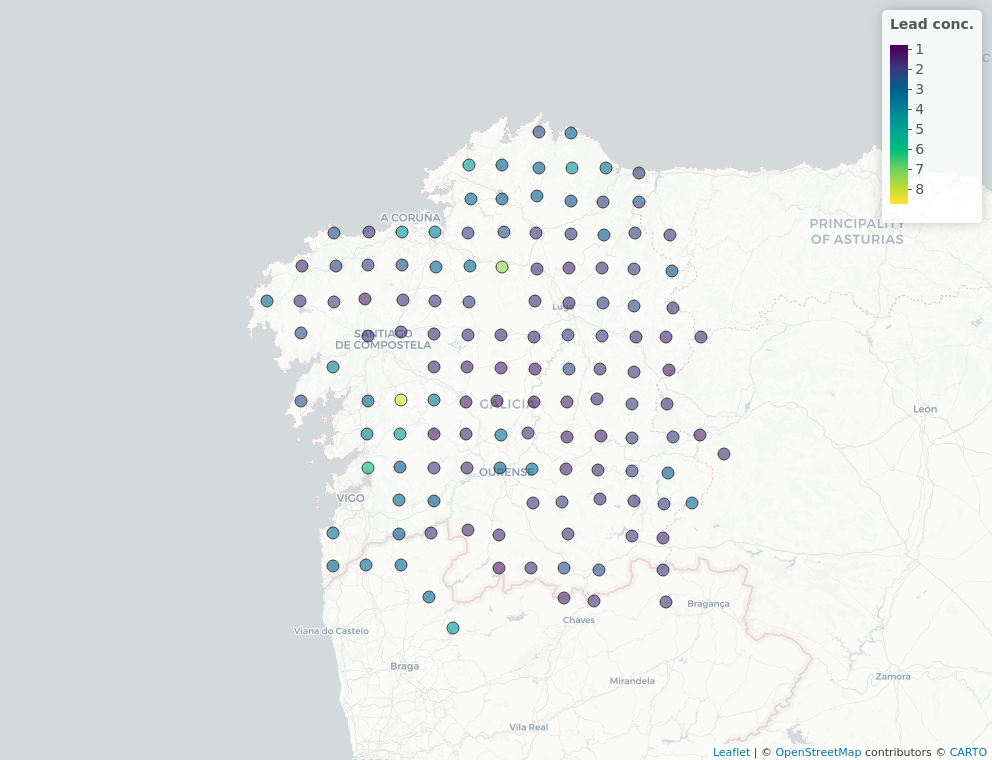
\includegraphics[width=3.31in,height=\textheight]{./figures/galicia_ch1.png}

}

\caption{\label{fig-galicia-ch1}Data on the meausred lead concentration
(in micrograms per gram dry weight) in moss samples collected in
Galicia, North-West of Spain.}

\end{figure}

Lead is a heavy metal which, in high concentrations, can cause chronic
damage to living organisms over a long period of time. For this reason
its spread and source must be regularly monitored. To assess the extent
of the contamination in an area, measurements of lead are often taken
from plants. The data here considered (Figure~\ref{fig-galicia-ch1})
consist of 132 locations of moss samples collected in 2000, in and
around Galicia, a region in the North-Western part of Spain. One of the
objectives of this survey was to establish the spatial pattern of lead
concentration in Galicia so as to better identify possible sources of
contamination; fore more information, see Fernández, Rey, and
Carballeira (2000).

In this case, geostatistical modelling can be used to predict the lead
concentration across Galicia and allows to disentangle variation which
is purely random, possibly due to measurement error, and genuine spatial
variation, which is our main object of interest.

This data-set will be used in this book to show how to carry out the
spatial analysis of continuously measured variables using linear
geostatistical models.

\hypertarget{river-blindness-in-liberia}{%
\subsection{River-blindness in
Liberia}\label{river-blindness-in-liberia}}

\begin{figure}

{\centering 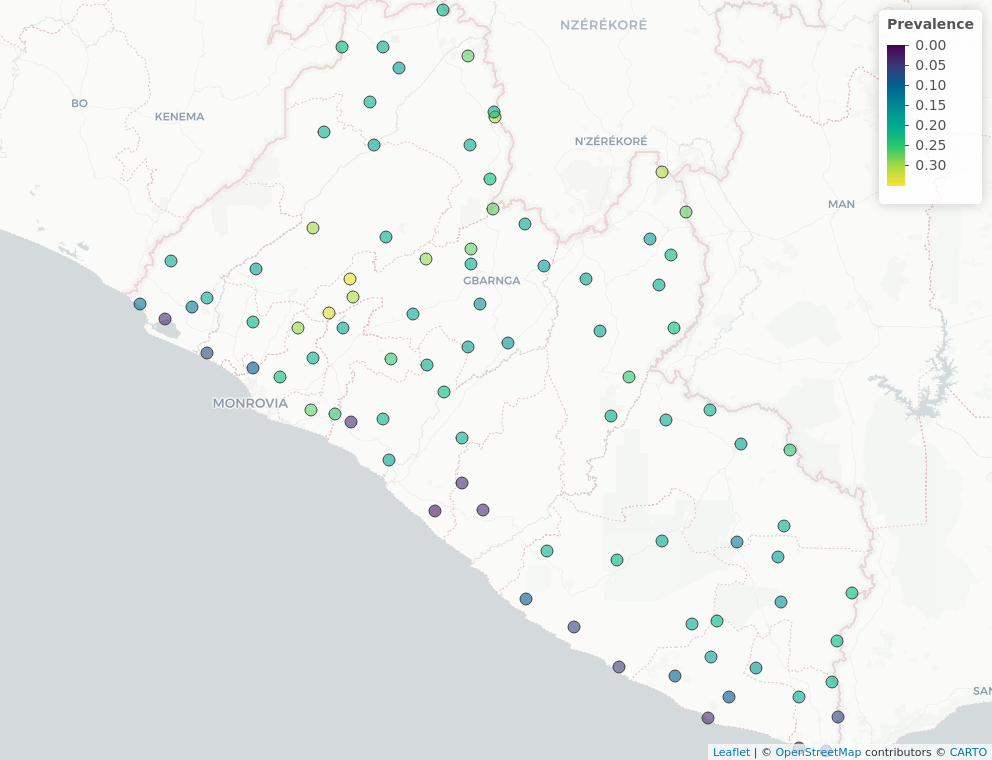
\includegraphics[width=3.31in,height=\textheight]{./figures/liberia_ch1.png}

}

\caption{\label{fig-liberia-ch1}River-blindness data from a
cross-sectional survey carried out in Liberia.}

\end{figure}

In low-resource settings, where disease registries are typically absent,
cross-sectional surveys are an essential monitoring tool that enables
the estimation of the disease burden in a population of interest. The
data considered in this example (Figure~\ref{fig-liberia-ch1}) have been
collected as part of an Africa-wide initiative called the Rapid
Epidemiological Mapping of Onchocerchiasis (REMO) carried out in 2011 in
20 African countries (Zouré et al. 2014). The goal of REMO is to
identify areas where river-blindness (or onchocerchiasis), a disease
transmitted by black flies who breed along fast flowing rivers, is still
a public health problem. In this context, it is especially of interest
to identify communities with a prevalence above 20\% and for treatment
is urgently needed.

In this book, we will use data collected from Liberia to model nodule
prevalence, which is based on a alternative and cheaper diagnostic
technique for river-blindness. In the analysis of this data-set, we will
illustrate how to formulate and fit Binomial geostatistical models, and
how these can be used to predict prevalence within a region of interest.

\hypertarget{malaria-in-the-western-kenyan-highlands}{%
\subsection{Malaria in the Western Kenyan
Highlands}\label{malaria-in-the-western-kenyan-highlands}}

\begin{figure}

{\centering 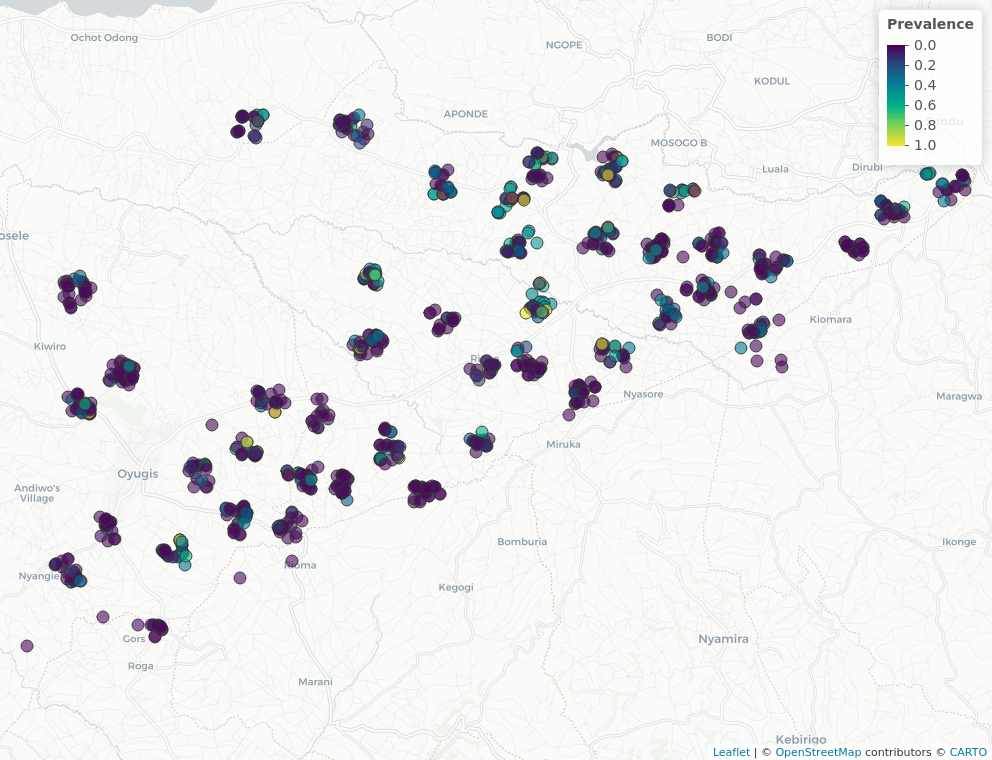
\includegraphics[width=3.31in,height=\textheight]{./figures/malkenya_ch1.png}

}

\caption{\label{fig-malkenya-ch1}\ldots{}}

\end{figure}

\hypertarget{anopheles-gambiae-mosquitoes-in-southern-cameroon}{%
\subsection{\texorpdfstring{\emph{Anopheles gambiae} mosquitoes in
Southern
Cameroon}{Anopheles gambiae mosquitoes in Southern Cameroon}}\label{anopheles-gambiae-mosquitoes-in-southern-cameroon}}

\begin{figure}

{\centering 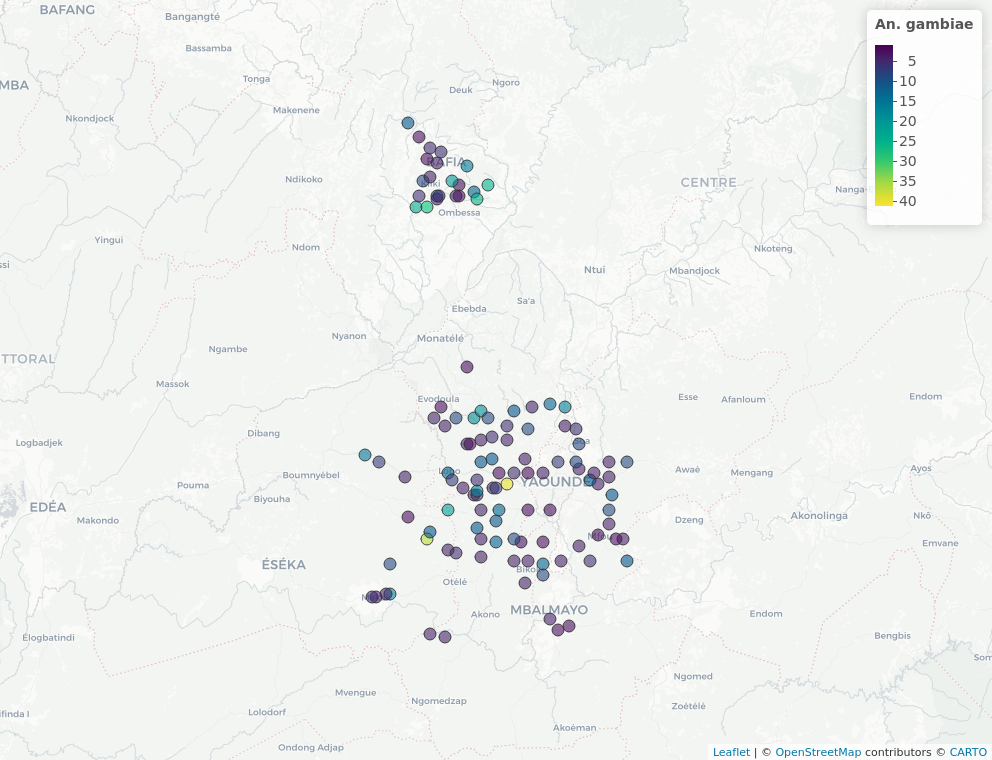
\includegraphics[width=3.31in,height=\textheight]{./figures/anopheles_ch1.png}

}

\caption{\label{fig-anopheles-ch1}Map of the collected number of
\emph{Anopheles gambiae} mosquitoes in an area of Southern Cameroon.}

\end{figure}

In studies of vector-borne and zoonotic diseases, understanding of the
vector distribution can help to better guide the decision-making process
for the implementation, monitoring and evaluation of control programmes.
\emph{Anopheles gambiae} mosquitoes are one of the main vectors for
malaria transmission in sub-Saharan Africa. Their distribution over
space is affected by several environmental and climatic factors,
including temperature, humidity and vegetation.

The data-set on mosquitoes (Figure~\ref{fig-anopheles-ch1}) that will
use in the book consists of a sub-set taken from a large database (Tene
Fossog et al. 2015). This was assembled in order to understand how the
environment affects the distribution of different species of
\emph{Anopheles} mosquitoes in sub-Saharan Africa. This example data-set
will be used to illustrate the application of Poisson geostatistical
models for mapping mosquitoes abundance.

\hypertarget{sec-geostat-models}{%
\section{Geostatistical problems and geostatistical
models}\label{sec-geostat-models}}

What the examples of the previous section have in common is that, in
each case, the goal of statistical analysis is to draw inferences on an
unobserved spatially continuous surface using data collected from a
finite set of locations. The lead concentration in Galicia, the
prevalence for river-blindness in Liberia and the abundance of \emph{A.
gambiae} mosquitoes in Cameroon can all be represented as spatially
continuous processes that originate from the combined effects of
environmental factors. We denote this class of inferential problems as
\emph{geostatistical problems} for which a solution can be found through
the development and application of suitable \emph{geostatistical
models}, which are the subject of this book.

As one can soon realize, geostatistical problems are not unique to
global health but arise in many other fields of science, including
economics, physics, biology, geology and others. It thus comes to no
surprise that geostatistics was initially developed in the South African
mining industry in the 1950s (Krige 1951). This was then further
developed as a self-contained discipline by Georges Matheron and other
researchers at Fontainebleau, in France (Matheron 1963; Chilès and
Delfiner 2016). In Watson (1971) and Watson (1972) a first connection is
drawn between geostatistics and the prediction of stochastic processes.
However, it is only with Ripley (1981) and then Cressie (1991) that
geostatistics is explicitly brought into a classical statistical
framework for the analysis of spatially referenced data. P. J. Diggle,
Tawn, and Moyeed (1998) coined the term \emph{model-based geostastics}
and introduced this as belonging to the general class of generalized
linear mixed models (Breslow and Clayton 1993), while emphasizing the
use of likelihood-based methods of inference. As in P. J. Diggle, Tawn,
and Moyeed (1998), also in this book, we advocate the application of
model-based geostistical models as a class of parametric statistical
models on which inference can be carried out using either maximum
likelihood estimation or Bayesian methods.

More precisely, our attention will be directed at the class of
\emph{generalized linear geostatistical models}, or GLGM. To formally
specify this, we first define the random variables \(S\), a spatial
stochastic process, and the random variable \(Y= (Y_1, \ldots, Y_n)\)
which correspond to the outcome observed at a set of locations
\(X = (x_1, \ldots, x_n)\). Let us use \([A]\) to denote ``the
distribution of the random variable \(A\)''. To formulate a GLGM, we
should then specify the joint distribution of \(S\) and \(Y\), which we
write as

\begin{equation}\protect\hypertarget{eq-glgm-joint-ch1}{}{
[Y, S] = [S] [Y | S].
}\label{eq-glgm-joint-ch1}\end{equation}

On the right-hand side of the equation above, we have factorized the
joint distribution of \(Y\) and \(S\), as the product between the
marginal distribution of \(S\) and the conditional distribution of \(Y\)
given \(S\). Hence, the formulation of a GLGM can be break down into the
tasks of formulating \([S]\) and \([Y | S]\).

In defining \([S]\), throughout the book, we shall assume that this is a
zero-mean stationary and isotropic Gaussian process. In other words,
these assumptions impose that the joint distribution of
\(S(X) = (S(x_1),\ldots,S(x_n))\), i.e.~the process \(S\) at the sampled
locations \(x_1, \ldots, x_n\), is invariant with respect to rations and
translations of the locations \(X\). In practical terms, the main
implication of this is that, for any pair of locations \(x_i\) and
\(x_j\) the correlation function \(\rho(\cdot)\) between \(S(x_i)\) and
\(S(x_j)\) is purely a function of the Euclidean distance, \(u_{ij}\),
between \(x_i\) and \(x_j\), i.e.

\begin{equation}\protect\hypertarget{eq-correlation-ch1}{}{
{\rm cov}\{S(x_i), S(x_j)\} = \sigma^2\rho(u_{ij}),
}\label{eq-correlation-ch1}\end{equation}

where \(\sigma^2\) is the variance of \(S(x)\) for all \(x\). In Chapter
3, we will look more closely at what type of correlation functions can
be used for \(\rho(\cdot)\) and how these affect our predictive
inferences. Furthermore, the fact that assume the process \(S\) to have
mean zero is because this is process acts as a residual term in our
modelling of \(Y\). This aspect will be reiterated several times in the
following chapters, as it as important implications for the
interpretation of the other components of a geostatistical model, as
well understanding the results of the analysis.

Finally, we model \([Y | S]\), i.e.~the distribution of \(Y\) given
\(S\), is modeled as a set of mutually independent distributions which
belong the exponential family, as defined in classical generalized
linear modelling framework (Nelder and Wedderburn 1972). It then follows
that, we can write \([Y | S]\) as

\begin{equation}\protect\hypertarget{eq-glm-ch1}{}{
[Y | S] = \prod_{i=1}^n [Y_i | S(x_i)].
}\label{eq-glm-ch1}\end{equation}

The final step then consists of specifying a distribution for
\([Y_i | S(x_i)]\). Table~\ref{tbl-glm} gives the range, mean and
variance the three specifications for \${[}Y\_i \textbar{}
S(x\_i){]}\$\$ which we will consider in this book. In
Table~\ref{tbl-glm}, the \emph{canonical function}, say \(g(\cdot)\),
denotes the natural transformation of the mean component \(\mu_i\) that
allows us to introduce both covariates and the spatial process
\(S(x_i)\) into the model so as to explain the variation in \(\mu_i\) as

\begin{equation}\protect\hypertarget{eq-linear-predictor-ch1}{}{
g(\mu_i) = d(x_i)^\top \beta + S(x_i).
}\label{eq-linear-predictor-ch1}\end{equation}

where \(d(x_i)\) is a vector of spatially referenced covariates with
associated regression coefficients \(\beta\). Finally, the quantity
\(m_i\), which appears in the formulation of the Binomial and Poisson
distributions, is an offset quantity and is used to account for the
number of \emph{tests} or the population size at a given location
\(x_i\).

\hypertarget{tbl-glm}{}
\begin{longtable}[]{@{}
  >{\raggedright\arraybackslash}p{(\columnwidth - 8\tabcolsep) * \real{0.2000}}
  >{\raggedright\arraybackslash}p{(\columnwidth - 8\tabcolsep) * \real{0.2000}}
  >{\raggedright\arraybackslash}p{(\columnwidth - 8\tabcolsep) * \real{0.2000}}
  >{\raggedright\arraybackslash}p{(\columnwidth - 8\tabcolsep) * \real{0.2000}}
  >{\raggedright\arraybackslash}p{(\columnwidth - 8\tabcolsep) * \real{0.2000}}@{}}
\caption{\label{tbl-glm}Type of outcomes \(Y_{i}\) considered in this
book.}\tabularnewline
\toprule\noalign{}
\begin{minipage}[b]{\linewidth}\raggedright
Distribution
\end{minipage} & \begin{minipage}[b]{\linewidth}\raggedright
Range of \(Y_i\)
\end{minipage} & \begin{minipage}[b]{\linewidth}\raggedright
Mean of \([Y_i | S(x_i)]\)
\end{minipage} & \begin{minipage}[b]{\linewidth}\raggedright
Variance of \([Y_i | S(x_i)]\)
\end{minipage} & \begin{minipage}[b]{\linewidth}\raggedright
Canonical link
\end{minipage} \\
\midrule\noalign{}
\endfirsthead
\toprule\noalign{}
\begin{minipage}[b]{\linewidth}\raggedright
Distribution
\end{minipage} & \begin{minipage}[b]{\linewidth}\raggedright
Range of \(Y_i\)
\end{minipage} & \begin{minipage}[b]{\linewidth}\raggedright
Mean of \([Y_i | S(x_i)]\)
\end{minipage} & \begin{minipage}[b]{\linewidth}\raggedright
Variance of \([Y_i | S(x_i)]\)
\end{minipage} & \begin{minipage}[b]{\linewidth}\raggedright
Canonical link
\end{minipage} \\
\midrule\noalign{}
\endhead
\bottomrule\noalign{}
\endlastfoot
Gaussian & \((-\infty, +\infty)\) & \(\mu_i\) & \(\tau^2\) &
\(g(\mu_i) = \mu_i\) \\
Binomial & \(1,\dots,m_i\) & \(m_i\mu_i\) & \(m_i\mu_i(1-\mu_i)\) &
\(g(\mu_i) = \log\{ \mu_i/(1-\mu_i) \}\) \\
Poisson & \(1,2,\ldots,\infty\) & \(m_i\mu_i\) & \(m_i\mu_i\) &
\(g(\mu_i) = \log\{ \mu_i \}\) \\
\end{longtable}

Based on the formulation in (\ref{eq-linear-predictor-ch1}), we can see
that \(S(x_i)\) quantifies residual spatial effects on \(\mu_i\) that
have not been accounted for by the covariates \(d(x_i)\). In an ideal
scenario, the covariates \(d(x_i)\) should explain all the spatial
variation without the need for \(S(x_i)\). Although this unrealistic, in
practice we may be able to most of the variation in \(\mu_i\) through
\(d(x_i)\) and, hence, reduce \(S(x_i)\) to a negligible component. In
Chapter 2, we will show how a thorough exploratory analysis can help to
understand whether we have come close to that ideal scenario or, if
instead, we need the use of GLGM to model the data.

The model described in (\ref{eq-linear-predictor-ch1}) can be seen as
the most basic GLGM that can be used for a geostatistical analysis. As
we will see in the analysis of some of the examples and, in Chapter 6,
for the case studies, extensions of this model will be required to
accommodate the intrinsic non-spatial random variation of the data which
is not captured by the covariates.

The types of problems that statistical models are applied to can be
distinguished into three main categories: prediction problems;
explanatory problems; problems of hypothesis testing. Most of the times,
geostatistical problems tend to fall under the first category, where the
goal is make predictive inferences on the process \(S(x)\) at location
\(x\), which is usually outside of the set of sampled locations.
However, as will illustrate in the later chapters, geostatistical models
play an important also in the other two types of problems. In
particular, we will show that spatial correlation can have a substantial
impact on the point estimates and standard errors for \(\beta\). Hence,
if the goal of the analysis is explain the relationship between a
covariate \(d(x)\) with the mean component \(\mu\).

\hypertarget{workflow-of-a-statistical-analysis-and-structure-of-the-book}{%
\section{Workflow of a statistical analysis and structure of the
book}\label{workflow-of-a-statistical-analysis-and-structure-of-the-book}}

\begin{figure}

{\centering 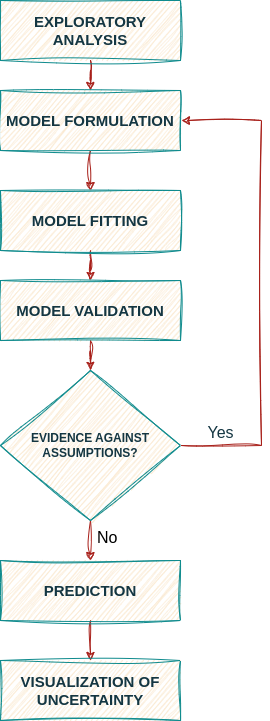
\includegraphics{./figures/workflow_diagram.png}

}

\caption{\label{fig-stages}Stages of a statistical analysis}

\end{figure}

Figure~\ref{fig-stages} shows the different stages that will follow in
carrying the geostatistical analysis of the examples introduced in
Section~\ref{sec-examples-ch1}. The exploratory analysis of the data is
an essential first step that is used to understand the empirical
associations between risk factors and the the health outcome of
interest. In our case, this first stage is also used to justify the use
of geostatistical models by questioning the underlying assumptions of
standard generalized linear models. Based on the results obtained from
the exploration of the data, we then formulate a suitable statistical
model and estimate its parameters using likelihood based methods of
inference. These also allows us to obtain uncertainty measures about the
strength of associations of regression relationships and the other model
parameters that define the shape of the spatial correlation in the data.
Following the estimation of the model, we then proceed to validate its
underlying assumptions using suitable diagnostics that assess whether
the model can later be sufficiently trusted to represent the observed
variation in the modelled outcome. At this stage, if the diagnostics
checks yield results that indicate the incompatibility of the model with
the data, we then back to the stage of model formulation and address the
issues arisen from the validation stage. If instead, we do not find any
evidence against the fitted model we can proceed to carry out sptatial
prediction. At this stage, it is important to define suitable predictive
targets that can help us to better answer the original research question
and better assist the decision making process. The final step of
visualization of uncertainty plays an important role in geostatistical
analysis in order to convey the main findings of the study in an
effective and easy-to-understand way for a wider audience which also
consists of non-experts.

In the remainder of this book, each chapter focuses on a specific stage
as shown in Figure~\ref{fig-stages}. We treat visualization of
uncertainty together with spatial prediction in Chapter 5.

Chapter 1 provides statistical methods for the exploration of
geostatistical data-sets, especially on the detection of residual
spatial correlation. In addition, we will also cover the handling and
visualization of spatial data in R. The skills learned in this will also
be useful in Chapter 5 and Chapter 6 for generating predictive maps of
the modelled outcome.

Chapter 2 focuses on the estimation of geostatistical models and will
provide an overview of Monte Carlo based methods for maximum likelihood
estimation.

Chapter 3 illustrated the use of methods that can be used to validate
the assumptions and calibration of statistical models.

Chapter 5 shows how geostatistical models can be used to carry out
spatial prediction of a health outcome of interest both on a spatially
continuous and spatially aggregated scales.

Finally, Chapter 6 presents the application of all the methods
illustrated in the previous chapters to three additional data-sets. This
chapter offers a summary of the content of book by putting together all
the stages in the geostatistical analyses for each of the three case
studies, and illustrates additional functionalities of the
\texttt{RiskMap} R package not covered in the previous chapters.

\bookmarksetup{startatroot}

\hypertarget{handling-of-spatial-data-in-r}{%
\chapter{Handling of spatial data in
R}\label{handling-of-spatial-data-in-r}}

This is a book created from markdown and executable code.

See (\textbf{knuth84?}) for additional discussion of literate
programming.

\begin{Shaded}
\begin{Highlighting}[]
\DecValTok{1} \SpecialCharTok{+} \DecValTok{1}
\end{Highlighting}
\end{Shaded}

\begin{verbatim}
[1] 2
\end{verbatim}

\hypertarget{importing-and-processing-spatial-data-in-r}{%
\section{Importing and processing spatial data in
R}\label{importing-and-processing-spatial-data-in-r}}

\hypertarget{visualizing-geostatistical-data}{%
\section{Visualizing geostatistical
data}\label{visualizing-geostatistical-data}}

\hypertarget{section}{%
\section{}\label{section}}

\bookmarksetup{startatroot}

\hypertarget{model-formulation-and-parameter-estimation}{%
\chapter{Model formulation and parameter
estimation}\label{model-formulation-and-parameter-estimation}}

\hypertarget{list-of-the-main-functions}{%
\section*{List of the main functions}\label{list-of-the-main-functions}}
\addcontentsline{toc}{section}{List of the main functions}

\markright{List of the main functions}

\begin{longtable}[]{@{}lll@{}}
\toprule\noalign{}
Function & R Package & Used for \\
\midrule\noalign{}
\endhead
\bottomrule\noalign{}
\endlastfoot
\texttt{lmer} & \texttt{lme4} & Fitting linear mixed models \\
\texttt{glmer} & \texttt{lme4} & Fitting generalized linear mixed
models \\
\texttt{glgm} & \texttt{RiskMap} & Fitting generalized linear mixed
models \\
\end{longtable}

\bookmarksetup{startatroot}

\hypertarget{exploratory-analysis}{%
\chapter{Exploratory analysis}\label{exploratory-analysis}}

As illustrated in Figure~\ref{fig-stages}, exploratory analysis is the
first step that should be carried out in a statistical analysis. This
stage is essential to inform how covariates should be introduced in the
model and, in our case, whether the variation unexplained by those
covariates exhibits spatial correlation.

In the exploratory analysis of count data, we will also look at how
overdispersion, which is a necessary, though not sufficient, condition
for residual spatial correlation.

\hypertarget{exploring-association-with-risk-factors}{%
\section{Exploring association with risk
factors}\label{exploring-association-with-risk-factors}}

Assessment of the association between the health outcome of interest and
non-categorical (i.e.~continuous) risk factors, can be carried through
scatter plots. The graphical exploration of the empirical association
between the outcome and the covariates is especially useful to identify
non-linear patterns in the relationship which should then be accounted
for in the model formulation.

Let us first consider the example of the river-blindess data in Liberia,
and examine the association between prevalence and elevation. We first
generate a plot of the prevalence against the measured elevation at each
of the sample locations

\begin{Shaded}
\begin{Highlighting}[]
\NormalTok{liberia}\SpecialCharTok{$}\NormalTok{logit }\OtherTok{\textless{}{-}}\NormalTok{ liberia}\SpecialCharTok{$}\NormalTok{npos}\SpecialCharTok{/}\NormalTok{liberia}\SpecialCharTok{$}\NormalTok{ntest}

\FunctionTok{ggplot}\NormalTok{(liberia, }\FunctionTok{aes}\NormalTok{(}\AttributeTok{x =}\NormalTok{ elevation, }\AttributeTok{y =}\NormalTok{ logit)) }\SpecialCharTok{+} \FunctionTok{geom\_point}\NormalTok{() }\SpecialCharTok{+}
  \FunctionTok{labs}\NormalTok{(}\AttributeTok{x=}\StringTok{"Elevation (meters)"}\NormalTok{,}\AttributeTok{y=}\StringTok{"Empirical logit"}\NormalTok{)}
\end{Highlighting}
\end{Shaded}

\begin{figure}[H]

{\centering 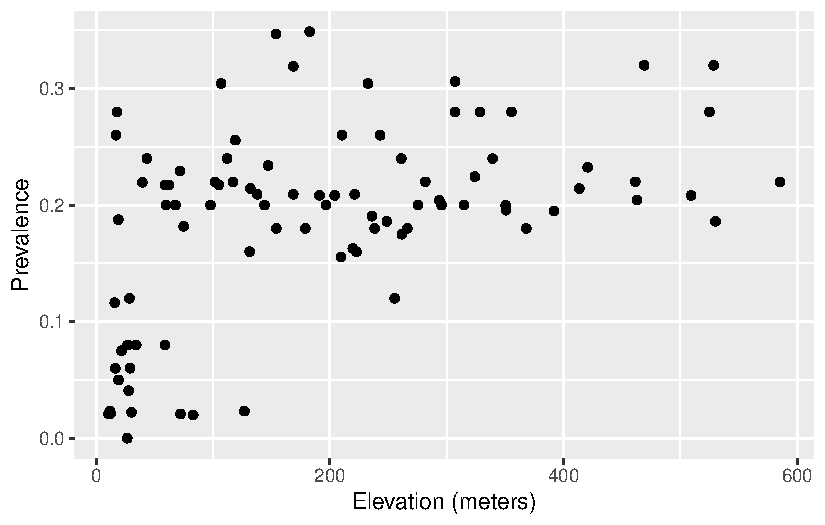
\includegraphics{03_model-fitting_files/figure-pdf/fig-prev-elev-liberia-1.pdf}

}

\caption{\label{fig-prev-elev-liberia}Scatter plot of the empirical
prevalence for river-blindess against elevation, measured in meters.}

\end{figure}

The plot shown in Figure~\ref{fig-prev-elev-liberia} shows that, when
elevation increases from 0 to around 100 meters, prevalence rapidly
increases to around 0.25 and, for larger values in elevation, the
relationship levels off. This begs the question of how we can account
for this in a regression model. However, the plot in
Figure~\ref{fig-prev-elev-liberia} cannot be used to inform this
decision because, when modelling prevalence data, regression
relationships are specified on the logit-transformed prevalence
(log-odds) scale; see Section Section~\ref{sec-geostat-models} . The
approach we follow to explore relationships in the case of prevalence
data is to the so called empirical logit, defined as

\begin{equation}\protect\hypertarget{eq-empirical-logit}{}{
e_{i} = \log\left\{\frac{y_i + 1/2}{n_i - y_i + 1/2}\right\}
}\label{eq-empirical-logit}\end{equation}

where \(y_i\) are the number of individuals who tested positive for
riverblindness and \(n_i\) is the total number of people tested at a
location. The reason for using the empirical logit, rather than the
standard logit transformation applied directly to the empirical
prevalence, is that it allows to generate finite values for empirical
prevalence values of 0 and 1, for which the standard logit function is
not defined.

\begin{Shaded}
\begin{Highlighting}[]
\FunctionTok{ggplot}\NormalTok{(liberia, }\FunctionTok{aes}\NormalTok{(}\AttributeTok{x =}\NormalTok{ elevation, }\AttributeTok{y =}\NormalTok{ logit)) }\SpecialCharTok{+} \FunctionTok{geom\_point}\NormalTok{() }\SpecialCharTok{+}
  \FunctionTok{labs}\NormalTok{(}\AttributeTok{x=}\StringTok{"Elevation (meters)"}\NormalTok{,}\AttributeTok{y=}\StringTok{"Empirical logit"}\NormalTok{) }\SpecialCharTok{+}
  \FunctionTok{stat\_smooth}\NormalTok{(}\AttributeTok{method =} \StringTok{"gam"}\NormalTok{, }\AttributeTok{formula =}\NormalTok{ y }\SpecialCharTok{\textasciitilde{}} \FunctionTok{s}\NormalTok{(x),}\AttributeTok{se=}\ConstantTok{FALSE}\NormalTok{)}\SpecialCharTok{+}
  \FunctionTok{stat\_smooth}\NormalTok{(}\AttributeTok{method =} \StringTok{"lm"}\NormalTok{, }\AttributeTok{formula =}\NormalTok{ y }\SpecialCharTok{\textasciitilde{}}\NormalTok{ x }\SpecialCharTok{+} \FunctionTok{I}\NormalTok{((x}\DecValTok{{-}150}\NormalTok{)}\SpecialCharTok{*}\NormalTok{(x}\SpecialCharTok{\textgreater{}}\DecValTok{150}\NormalTok{)),}
              \AttributeTok{col=}\StringTok{"red"}\NormalTok{,}\AttributeTok{lty=}\StringTok{"dashed"}\NormalTok{,}\AttributeTok{se=}\ConstantTok{FALSE}\NormalTok{) }\SpecialCharTok{+}
  \FunctionTok{stat\_smooth}\NormalTok{(}\AttributeTok{method =} \StringTok{"lm"}\NormalTok{, }\AttributeTok{formula =}\NormalTok{ y }\SpecialCharTok{\textasciitilde{}} \FunctionTok{log}\NormalTok{(x),}
              \AttributeTok{col=}\StringTok{"green"}\NormalTok{,}\AttributeTok{lty=}\StringTok{"dashed"}\NormalTok{,}\AttributeTok{se=}\ConstantTok{FALSE}\NormalTok{)}
 
\end{Highlighting}
\end{Shaded}

\begin{figure}[H]

{\centering 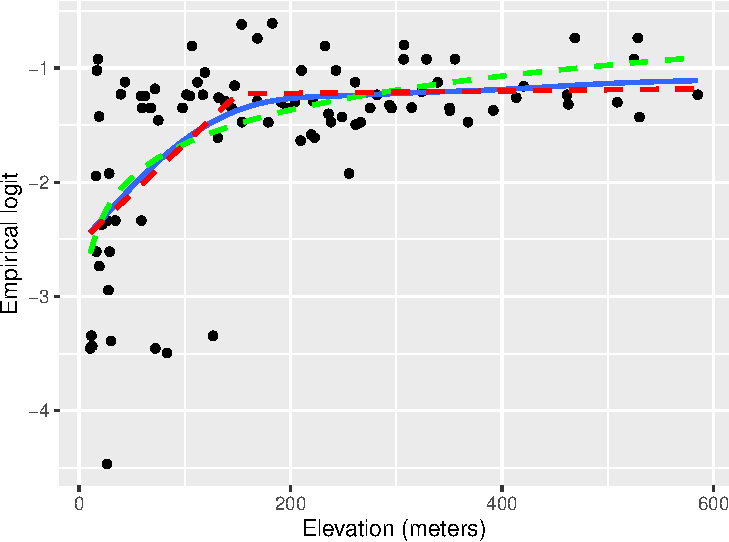
\includegraphics{03_model-fitting_files/figure-pdf/fig-elogit-elev-liberia-1.pdf}

}

\caption{\label{fig-elogit-elev-liberia}Scatter plot of the empirical
prevalence for river-blindess against elevation, measured in meters.}

\end{figure}

\hypertarget{exploring-overdispersion-in-count-data}{%
\section{Exploring overdispersion in count
data}\label{exploring-overdispersion-in-count-data}}

\hypertarget{exploring-residual-spatial-correlation}{%
\section{Exploring residual spatial
correlation}\label{exploring-residual-spatial-correlation}}

\bookmarksetup{startatroot}

\hypertarget{linear-gaussian-model}{%
\chapter{Linear Gaussian model}\label{linear-gaussian-model}}

\bookmarksetup{startatroot}

\hypertarget{generalized-linear-geostatistical-models}{%
\chapter{Generalized linear geostatistical
models}\label{generalized-linear-geostatistical-models}}

\bookmarksetup{startatroot}

\hypertarget{model-validation}{%
\chapter{Model validation}\label{model-validation}}

This is a book created from markdown and executable code.

See (\textbf{knuth84?}) for additional discussion of literate
programming.

\begin{Shaded}
\begin{Highlighting}[]
\DecValTok{1} \SpecialCharTok{+} \DecValTok{1}
\end{Highlighting}
\end{Shaded}

\begin{verbatim}
[1] 2
\end{verbatim}

\hypertarget{how-to-simulate-geostatistical-data-from-a-fitted-model}{%
\section{How to simulate geostatistical data from a fitted
model}\label{how-to-simulate-geostatistical-data-from-a-fitted-model}}

\hypertarget{validating-the-calibration-of-the-model}{%
\section{Validating the calibration of the
model}\label{validating-the-calibration-of-the-model}}

\hypertarget{validating-the-spatial-correlation-of-the-model}{%
\section{Validating the spatial correlation of the
model}\label{validating-the-spatial-correlation-of-the-model}}

\bookmarksetup{startatroot}

\hypertarget{geostatistical-prediction}{%
\chapter{Geostatistical prediction}\label{geostatistical-prediction}}

This is a book created from markdown and executable code.

See (\textbf{knuth84?}) for additional discussion of literate
programming.

\begin{Shaded}
\begin{Highlighting}[]
\DecValTok{1} \SpecialCharTok{+} \DecValTok{1}
\end{Highlighting}
\end{Shaded}

\begin{verbatim}
[1] 2
\end{verbatim}

\hypertarget{pixel-level-predictive-targets}{%
\section{Pixel-level predictive
targets}\label{pixel-level-predictive-targets}}

\hypertarget{area-level-predictive-targets}{%
\section{Area-level predictive
targets}\label{area-level-predictive-targets}}

\hypertarget{comparing-the-predictive-performance-of-geostatistical-models}{%
\section{Comparing the predictive performance of geostatistical
models}\label{comparing-the-predictive-performance-of-geostatistical-models}}

\bookmarksetup{startatroot}

\hypertarget{case-studies}{%
\chapter{Case studies}\label{case-studies}}

This is a book created from markdown and executable code.

See (\textbf{knuth84?}) for additional discussion of literate
programming.

\begin{Shaded}
\begin{Highlighting}[]
\DecValTok{1} \SpecialCharTok{+} \DecValTok{1}
\end{Highlighting}
\end{Shaded}

\begin{verbatim}
[1] 2
\end{verbatim}

\hypertarget{mapping-stunting-risk-in-ghan}{%
\section{Mapping stunting risk in
Ghan}\label{mapping-stunting-risk-in-ghan}}

\hypertarget{mapping-river-blindness-in-malawi}{%
\section{Mapping river blindness in
Malawi}\label{mapping-river-blindness-in-malawi}}

\hypertarget{mapping-mosquitoes-abundance-in-cameroon}{%
\section{Mapping mosquitoes abundance in
Cameroon}\label{mapping-mosquitoes-abundance-in-cameroon}}

\bookmarksetup{startatroot}

\hypertarget{references}{%
\chapter*{References}\label{references}}
\addcontentsline{toc}{chapter}{References}

\markboth{References}{References}

\hypertarget{refs}{}
\begin{CSLReferences}{1}{0}
\leavevmode\vadjust pre{\hypertarget{ref-breslow1993}{}}%
Breslow, N. E., and D. G. Clayton. 1993. {``Approximate Inference in
Generalized Linear Mixed Models.''} \emph{Journal of the American
Statistical Association} 88: 9--25.

\leavevmode\vadjust pre{\hypertarget{ref-chilesdelfiner2016}{}}%
Chilès, J-P, and P. Delfiner. 2016. \emph{Geostatistics (Second
Edition)}. Hoboken: Wiley.

\leavevmode\vadjust pre{\hypertarget{ref-cressie1991}{}}%
Cressie, N. A. C. 1991. \emph{Statistics for Spatial Data}. New York:
Wiley.

\leavevmode\vadjust pre{\hypertarget{ref-diggle1998}{}}%
Diggle, P. J., J. A. Tawn, and R. A. Moyeed. 1998. {``Model-Based
Geostatistics.''} \emph{Journal of the Royal Statistical Society: Series
C (Applied Statistics)} 47 (3): 299--350.
\url{https://doi.org/10.1111/1467-9876.00113}.

\leavevmode\vadjust pre{\hypertarget{ref-diggleBook2019}{}}%
Diggle, Peter J. 2019. \emph{Model-Based Geostatistics for Global Public
Health : Methods and Applications.} Chapman and Hall/CRC
Interdisciplinary Statistics Ser. Milton: Chapman; Hall/CRC.

\leavevmode\vadjust pre{\hypertarget{ref-dobson2008}{}}%
Dobson, A. J., and A. Barnett. 2008. \emph{An Introduction to
Generalized Linear Models}. Third. Chapman; Hall/CRC.

\leavevmode\vadjust pre{\hypertarget{ref-fernandez2000}{}}%
Fernández, J. A, A Rey, and A Carballeira. 2000. {``An Extended Study of
Heavy Metal Deposition in Galicia (NW Spain) Based on Moss Analysis.''}
\emph{Science of The Total Environment} 254 (1): 31--44.
\url{https://doi.org/10.1016/S0048-9697(00)00431-9}.

\leavevmode\vadjust pre{\hypertarget{ref-krige1951}{}}%
Krige, D. G. 1951. {``A Statistical Approach to Some Basic Mine
Valuation Problems on the Witwatersrand.''} \emph{Journal of the
Chemical, Metallurgical and Mining Society of South Africa} 52: 119--39.

\leavevmode\vadjust pre{\hypertarget{ref-matheron1963}{}}%
Matheron, G. 1963. {``Principles of Geostatistics.''} \emph{Economic
Geology} 58: 1246--66.

\leavevmode\vadjust pre{\hypertarget{ref-nelder1972}{}}%
Nelder, J. A., and R. W. M. Wedderburn. 1972. {``Generalized Linear
Models.''} \emph{Journal of the Royal Statistical Society A} 135:
370--84.

\leavevmode\vadjust pre{\hypertarget{ref-pawitan2001}{}}%
Pawitan, Yudi. 2001. \emph{In All Likelihood : Statistical Modelling and
Inference Using Likelihood}. Oxford ; New York: Clarendon Press : Oxford
University Press.

\leavevmode\vadjust pre{\hypertarget{ref-ripley1981}{}}%
Ripley, B. D. 1981. \emph{Spatial Statistics}. New York: Wiley.

\leavevmode\vadjust pre{\hypertarget{ref-ross2013}{}}%
Ross, Sheldon. 2013. \emph{First Course in Probability, a.} 9th ed.
Harlow: Pearson Education UK.

\leavevmode\vadjust pre{\hypertarget{ref-fossog2015}{}}%
Tene Fossog, Billy, Diego Ayala, Pelayo Acevedo, Pierre Kengne, Ignacio
Ngomo Abeso Mebuy, Boris Makanga, Julie Magnus, et al. 2015. {``Habitat
Segregation and Ecological Character Displacement in Cryptic African
Malaria Mosquitoes.''} \emph{Evolutionary Applications} 8 (4): 326--45.
\url{https://doi.org/10.1111/eva.12242}.

\leavevmode\vadjust pre{\hypertarget{ref-watson1971}{}}%
Watson, G. S. 1971. {``Trend -Surface Analysis.''} \emph{Mathematical
Geology} 3: 215--26.

\leavevmode\vadjust pre{\hypertarget{ref-watson1972}{}}%
---------. 1972. {``Trend Surface Analysis and Spatial Correlation.''}
\emph{Geological Society of America Special Paper} 146: 39--46.

\leavevmode\vadjust pre{\hypertarget{ref-zoure2014}{}}%
Zouré, Honorat GM, Mounkaila Noma, Afework H Tekle, Uche V Amazigo,
Peter J Diggle, Emanuele Giorgi, and Jan HF Remme. 2014. {``Geographic
Distribution of Onchocerciasis in the 20 Participating Countries of the
African Programme for Onchocerciasis Control: (2) Pre-Control Endemicity
Levels and Estimated Number Infected.''} \emph{Parasites \& Vectors} 7
(1): 326--26.

\end{CSLReferences}



\end{document}
